\documentclass[12pt,english]{article}
\usepackage{setspace}
\doublespacing
\usepackage[affil-it]{authblk}
\usepackage{graphicx}
\usepackage[space]{grffile}
\usepackage{latexsym}
\usepackage{textcomp}
\usepackage{longtable}
\usepackage[flushleft]{threeparttable} 
\usepackage{multirow,booktabs}
\usepackage{ltablex,array} % to scale longtables
\usepackage{lipsum}
\usepackage{amsfonts,amsmath,amssymb}
\usepackage{url}
\usepackage[utf8]{inputenc}
\usepackage{hyperref}
\hypersetup{colorlinks=false,pdfborder={0 0 0}}
\newcommand{\truncateit}[1]{\truncate{0.8\textwidth}{#1}}
\newcommand{\scititle}[1]{\title[\truncateit{#1}]{#1}}
\usepackage[T1]{fontenc}
\usepackage{caption} %have period instead of colon for figures and Table captions
\captionsetup[table]{labelsep=period}
\usepackage{nopageno}
  
\providecommand{\tabularnewline}{\\}
\usepackage[nolist]{acronym}
\newacro{BMI} {body mass index}  
\newacro{LMIC} {low- and middle-income country}
\acrodefplural{LMIC}[LMICs]{low- and middle-income countries}  
\newacro{MIC} {middle-income country}
\acrodefplural{MIC}[MICs]{middle-income countries}  
\newacro{HIC} {high-income country}  
\acrodefplural{HIC}[HICs]{high-income countries}
\newacro{FE} {fixed effects}  
\newacro{HbA1c} {glycated hemoglobin}  
\newacro{IDF} {International Diabetes Federation}  
\newacro{IV} {instrumental variable}  
\newacro{LPM} {linear probability model}  
\newacro{MxFLS} {Mexican Family Life Survey}  
\newacro{OLS} {ordinary least squares}  
\newacro{RE} {random effects}
\newacro{p.p.} {percentage points}    
\newacro{US} {United States}
\newacro{WHO} {World Health Organization} 
\newacro{WB} {within-between} 
\newacro{USA} {United States of America}   
\usepackage{longtable}
\usepackage{booktabs}
\usepackage{multirow}
\usepackage{graphicx}
\usepackage[Export]{adjustbox}
%landscape pages
\usepackage{pdflscape}
\newcommand{\comment}[1]{}  %allows multiline comments
\usepackage[english]{babel}% Recommended
\usepackage{csquotes}
\usepackage{lineno} %line numbers
%\linenumbers
\usepackage[
maxcitenames=2, 
style=authoryear-comp,
firstinits=true,
maxbibnames=99,
backend=biber,
uniquename=false,
url=false,
isbn=false,
doi=true]{biblatex}
%\DeclareLanguageMapping{english}{english-apa}
\DeclareNameAlias{sortname}{first-last}
%\renewcommand*{\nameyeardelim}{\addcomma\space}


\AtEveryBibitem{\clearfield{month}}
	
\addbibresource{/home/till/Dokumente/BibTex/Second_Mexico_paper.bib}

%SPECIFIC FORMATING RULES OF JOURNAL

\renewcommand{\thesection}{\arabic{section}.}
\renewcommand{\thesubsection}{\thesection\arabic{subsection}.}





% paper margins
\usepackage{geometry}
\geometry{
letterpaper,
left=25mm,
right=30mm,
top=20mm,
bottom=30mm,
}   
%limiting tables to only float within section
\usepackage{placeins}
  
  
% formating

\usepackage{listings}
\lstset{ %
  backgroundcolor=\color{white},   % choose the background color
  basicstyle=\footnotesize,        % size of fonts used for the code
  breaklines=true,                 % automatic line breaking only at whitespace
  captionpos=b,                    % sets the caption-position to bottom
  commentstyle=\color{OliveGreen},    % comment style
  keywordstyle=\color{BlueViolet},       % keyword style
  stringstyle=\color{black},     % string literal style
  language=[AlLaTeX]TeX,             % Set your language (you can change the language for each code-block optionally)
  frame=lrtb, %
  xleftmargin=\fboxsep, %
  xrightmargin=-\fboxsep, %
  moretexcs={lstset,color,colorlet, cellcolor, newcolumntype, columncolor, rowcolor, multirow, xspace, LaTeX, TeX},
}

	% *****************************************************************
	% siunitx
	% *****************************************************************
\usepackage{siunitx} % centering in tables
\sisetup{
	detect-mode,
	tight-spacing		= true,
	group-digits		= false ,
	input-signs		= ,
	input-symbols		= ( ) [ ] - + *,
	input-open-uncertainty	= ,
	input-close-uncertainty	= ,
	table-align-text-post	= false
}

	        
	        
%For Table commands to change column sizeand alignment, especially tabularx
\newcolumntype{b}{X}  %large columns http://tex.stackexchange.com/questions/84400/Table-layout-with-tabularx-column-widths-502525
\newcolumntype{m}{>{\hsize=.5\hsize}X} % medium columns
\newcommand{\merge}[1]{\multicolumn{2}{>{\hsize=\dimexpr2\hsize+2\tabcolsep+\arrayrulewidth\relax}X}{#1}}  %allows merging of two columns in tabularx http://tex.stackexchange.com/questions/236155/tabularx-and-multicolumn

\newcolumntype{Y}{>{\centering\arraybackslash}X} %new columntype for X columns in tabularx to center them http://tex.stackexchange.com/questions/89166/centering-in-tabularx-and-x-columns
\newcolumntype{Z}{>{\raggedright\let\newline\\\arraybackslash\hspace{0pt}}X} %left aligned X columns http://tex.stackexchange.com/questions/97180/how-to-get-column-alignment-in-tabularx
\newcolumntype{z}{>{\hsize=.5\hsize\\\raggedright\let\newline\\\arraybackslash\hspace{0pt}}X} %left aligned X columns http://tex.stackexchange.com/questions/97180/how-to-get-column-alignment-in-tabularx
\newcolumntype{y}{>{\hsize=.5\hsize}Y} % small columns


        


\makeatletter
\def\@maketitle{%
	\newpage
	\null
	\vskip 2em%
	\begin{center}%
		\let \footnote \thanks
		{\Large\bfseries \@title \par}%
		\vskip 1.5em%
		{\normalsize
			\lineskip .5em%
			\begin{tabular}[t]{c}%
				\@author
			\end{tabular}\par}%
		\vskip 1em%
		{\normalsize \@date}%
	\end{center}%
	\par
	\vskip 1.5em}
\makeatother        
\begin{document}
	\title{The impact of diabetes on labour market outcomes in Mexico: a panel data and biomarker analysis}
	\author{}
	\date{}
	\maketitle 
	\thispagestyle{empty}
	\clearpage

	
\begin{abstract}
Recent evidence for Mexico suggests important differences in health status between people with diagnosed and undiagnosed diabetes. However, there is at best scarce evidence on the economic consequences of diabetes, especially in contexts where the condition often remains undiagnosed, as is typically the case in low- and middle income countries. Using Mexican longitudinal as well as biomarker data we estimated the impact of diabetes and diabetes duration on employment probabilities, wages and working hours. We further explored how these effects differed for those aware and those unaware of their diabetes. For the longitudinal analyses nationally representative data from 11836 men and 13745 women 15 to 64 years old were taken from three waves (2002, 2005, 2009) of the Mexican Family Life Survey. We estimated a within-between effects model to account for unmeasured time-invariant confounders of diabetes while simultaneously assessing differences between subjects with and without diabetes. The within effects indicated a reduction in the probability of being employed between 5.4 and 6.0 percentage points for men and women, respectively, but no effects on hours worked or wages. The between effects showed similar results. Employment probabilities fell gradually with each year since diagnosis. Using cross-sectional biomarker data, we observed that 68\% of those exhibiting glycated hemoglobin (HbA1c) levels above the clinical diabetes threshold did not self-report a diagnosis, hence were undiagnosed. Nevertheless, regression analysis revealed that there was no association of diabetes with labour outcomes for undiagnosed women or men. This suggests that results based on self-reported diabetes cannot be extended to the considerable population with undiagnosed diabetes, likely because of a selection of people in worse health and with a longer diabetes duration into the diagnosed population. An earlier diagnosis and improved treatment of diabetes therefore may prevent adverse health effects and related economic hardship in Mexico.
\end{abstract}


\section{\label{sec:Introduction}Introduction }

Diabetes, a disease characterized by elevated blood glucose levels due to the body's inability to use insulin properly, has in the last two decades increasingly become a problem for \acp{LMIC} as well as \acp{HIC}, with over two-thirds of people with diabetes living in the developing world \parencite{InternationalDiabetesFederation2015}. In Mexico, diabetes prevalence is estimated to have grown from 6.7\% in 1994 to 14.4\% in 2006 \parencite{Barquera2013} and 15.8\% in 2015. Diabetes has become the number one contributor to mortality \parencite{InternationalDiabetesFederation2015}, by increasing the risk for heart disease and stroke, blindness, kidney disease and nerve problems, food ulcers and amputations \parencite{Reynoso-Noveron2011}. However, via effective self-management of the disease, many if not all of the complications can be avoided \parencite{Lim2011, Gregg2012}.

The observed increase in diabetes incidence has been attributed to a deterioration in diet and a reduction in physical activity \parencite{Barquera2008b,Basu2013}, while genetic predisposition among Mexicans with pre-Hispanic ancestry may also play a role \parencite{Williams2013}. The onset of diabetes has been occurring at an ever earlier age in Mexico \parencite{Bello-Chavolla2017a}, increasing the risk of complications occurring during the productive lifespan. Only a minority of patients in Mexico achieves adequate blood glucose control \parencite{Barquera2013}. Moreover, diabetes in Mexico coexist with high levels of infectious diseases, exposing the health system to a 'double-disease burden' increasing the pressure to identify treatment priorities and use existing resources efficiently\parencite{Gutierrez-delgado2009}.

Despite the catastrophic impact of diabetes on health, its economic consequences, in particular in \acp{LMIC} have received less attention, especially its effects on labour outcomes \parencite{Anonymous2007}. The latter have been studied predominantly in high-income countries, where substantial economic losses have been observed \parencite{Brown2005,Brown2014,BrownIII2011,Minor2011,Minor2013,Minor2015,Latif2009}. For \acp{LMIC} less evidence is available. One study exploited a natural experiment in China and found a significant reduction in income due to a recent diabetes diagnosis \parencite{Liu2014}. A study for Mexico, using cross-sectional data from 2005, found a significant (p<0.01) reduction in employment probabilities for males by 10 \ac{p.p.} and for females by 4.5 \ac{p.p.} (p<0.1) \parencite{Anonymous2007}. Most existing studies rely on \ac{IV} estimation to address the potential endogeneity of diabetes using the genetic component of diabetes based on its family history as an instrument.  However, family history of diabetes may also proxy for other genetically transferred traits, including unobserved abilities, as well as  intrahousehold or intergenerational dynamics that impact labour outcomes directly; the validity of this \ac{IV} therefore remains debatable. Panel data methods provide the opportunity to account for time-invariant unobserved individual characteristics, which may play an important role, but have not yet been used by our knowledge. Such unobservables, like for instance health endowments could adversely affect health as well as the propensity to develop type 2 diabetes in particular \parencite{VanEwijk2011,Sotomayor2013,Li2010b}; they may also affect labour outcomes---either directly through their effects on contemporaneous productivity \parencite{Currie2013}, or indirectly by limiting educational attainment and human capital accumulation \parencite{Ayyagari2011a}. These unobservables thereby present a major source of a potential bias that can be accounted for by the use of panel data estimation.

In parallel to these identification challenges, heterogeneity in impact and measurement across the population also deserves further investigation. Recent evidence from Mexico points to a strong positive relationship of diabetes duration with mortality due to diabetes related complications \parencite{Herrington2018}. A longer disease duration was found to be related with higher \ac{HbA1c} levels and undiagnosed diabetes had the lowest diabetes related mortality risks. The latter points to potential selection issues when using self-reported diabetes data to investigate economic outcomes as those who self-report, and hence tend to be diagnosed, are in worse health than those undiagnosed, potentially leading to an overestimation of the economic effects of diabetes, in particular in populations with a large undiagnosed population, such as in many \acp{LMIC} \parencite{Beagley2014}. So far, however, little evidence exists on the economic impact according to diabetes severity and duration or for those with undiagnosed diabetes. 

The objective of this study was to provide new evidence on the impact of diabetes on labour outcomes, adding to previous work by paying close attention to the challenges of unobserved heterogeneity, to the chronic nature of diabetes and to the population unaware of their condition (i.e. the 'undiagnosed'). We used three waves of Mexican panel data, covering the period 2002--2012. Applying a within-between model, which  models individual fixed effects and between effects separately, we accounted for time-invariant heterogeneity when assessing the impact of self-reported diabetes and time since diagnosis on labour outcomes. We also used rich and novel biomarker data from the most recent wave of data, we assessed the role of undiagnosed diabetes.

\section{\label{sec:Data}Data}

This paper uses data from the \acf{MxFLS}, a nationally representative longitudinal household survey, containing three waves conducted in 2002, 2005--2006 and 2009--2012. Data was collected on a wide range of social, demographic, economic and health characteristics \parencite{Rubalcava2013}. Our samples were restricted to the working age population (15--64) and excluded pregnant women and those in school. Pregnant women have an increased diabetes risk and may not be able to work. Since their inclusion may have biased the estimates we dropped all observations of women reporting to be pregnant at the time of the survey (N=764). The first part of the analysis used all three waves and the panel structure of the data. The second part used a biomarker subsample of the third wave (2009--2012). Because the biomarker sample included everybody above the age of 44 but only a random subsample of those aged 44 or below \parencite{Crimmins2015}, its age structure was older and hence its self-reported diabetes prevalence higher. The analysis therefore compares with self-reported data for this specific subsample only.

Our outcome variables of interest were employment status, weekly working hours, hourly wage, and occupation. Employment status was defined as having carried out an activity that helped with the household expenses the last week and working for at least four hours per week. We explicitly included informal employment and employment without monetary remuneration, for instance in family businesses.  Hourly wage was constructed as reported monthly income from the first and second job, divided by average number of weeks per month and weekly working hours.  Labour income was obtained from the response to questions on wages, income from piecework, tips, income from extra hours, meals, housing, transport, medical benefits and other earnings, or from the response to a question on aggregate labour income for the entire month. We adjusted calculated wages for inflation in the year of interview and considered the log of real wages. Due to a considerable number of missing or zero income reports, the sample used for the wage estimation was smaller than the sample for working hours. Working hours were combined from both the first and a potential second job. Descriptive statistics for the entire panel sample show that 86\% of men reported some form of employment compared to 37\% of women (see Table \ref{tab:Pooled-sample-characteristics}). Interestingly, men did not report considerably higher hourly wages than women but worked more hours per week. Men also more often worked in agricultural jobs while women were more likely to be self-employed or in non-agricultural wage employment. The educational attainment of women was lower than that for men on average.

\begin{table}[!ht]
	\caption{\label{tab:Pooled-sample-characteristics}{\bf Descriptive statistics for the panel sample (2002,2005,2009).}}
	
	\begin{adjustbox}{max width=\linewidth, center}
		\begin{threeparttable}  %adds notes to tables
			{
				\def\sym#1{\ifmmode^{#1}\else\(^{#1}\)\fi}
				\begin{tabular}{l*{6}{S S}}
					\toprule
					&\multicolumn{3}{c}{Males}             &\multicolumn{3}{c}{Females}\\\cmidrule(lr){2-4}\cmidrule(lr){5-7}         
					&\multicolumn{1}{c}{No diabetes}&\multicolumn{1}{c}{Diabetes}&  \multicolumn{1}{c}{p (t-test)}&\multicolumn{1}{c}{No diabetes}&\multicolumn{1}{c}{Diabetes}&  \multicolumn{1}{c}{p (t-test)}\\
					\midrule
					\hspace*{10mm}\emph{Dependent variables} \\
					Employed            &        0.87&        0.80&        0.00&        0.37&        0.26&        0.00\\
					Hourly wage  (in Mexican Peso)       &       42.29&       46.79&        0.83&       40.67&       36.33&        0.61\\
					Weekly working hours&       46.83&       46.51&        0.60&       39.06&       37.51&        0.09\\
					Non-agricultural worker or employee&        0.51&        0.41&        0.00&        0.24&        0.13&        0.00\\
					Agricultural worker&        0.19&        0.13&        0.00&        0.02&        0.01&        0.00\\
					Self-employed&        0.16&        0.26&        0.00&        0.09&        0.11&        0.04\\
					\hspace*{10mm}\emph{Diabetes variables} \\
					Diabetes duration (years)   &  &        7.40&        &        &        7.79&        \\
					\hspace*{10mm}\emph{Control variables} \\
					Age                 &       35.31&       50.68&        0.00&       35.37&       50.45&        0.00\\
					Any medical insurance&        0.47&        0.59&        0.00&        0.50&        0.62&        0.00\\
					City of 2,5oo-15,000&        0.11&        0.09&        0.03&        0.11&        0.13&        0.00\\
					City of 15,000-100,000&        0.10&        0.14&        0.00&        0.10&        0.10&        0.40\\
					City of >100,000    &        0.34&        0.39&        0.00&        0.35&        0.34&        0.47\\
					Married             &        0.53&        0.77&        0.00&        0.53&        0.66&        0.00\\
					Number of children (age<6) in household&        1.49&        1.14&        0.00&        1.60&        1.13&        0.00\\
					Indigenous group    &        0.19&        0.15&        0.00&        0.19&        0.19&        0.86\\
					Education &&&&&& \\                    
					\hspace*{10mm}Secondary           &        0.31&        0.22&        0.00&        0.31&        0.16&        0.00\\
					\hspace*{10mm}High school         & 0.16&        0.07&        0.00&        0.14&        0.03&        0.00\\
					\hspace*{10mm}Higher education    & 0.11&        0.12&        0.39&        0.10&        0.03&        0.00\\
					Wealth index        &        0.00&        0.04&        0.27&       -0.01&        0.01&        0.36\\
					N &20391&994&&25664&1666&\\
					\bottomrule
				\end{tabular}
				\begin{tablenotes}
					\item \footnotesize \textit{Notes} Mean values. Diabetes refers to self-reported diabetes.
				\end{tablenotes}
			}
		\end{threeparttable}
	\end{adjustbox}
\end{table}

The first part of the analysis focused on the relationship of labour outcomes with self-reported diabetes, which was based on the survey question: “Have you ever been diagnosed with diabetes?”. Because the data did not distinguish between type 1 and type 2 diabetes, we assumed that the estimates represented the impact of type 2 diabetes, by far the most common type of diabetes in Mexico. As a robustness check, we re-estimated our main results categorizing diabetes into early-onset and late-onset cases, according to the age at which diabetes was first reported in the survey. This was a similar approach to \textcite{Alegre-Diaz2016}, who assumed that everybody diagnosed before age 35 and using insulin had type 1 diabetes. Accordingly, we assumed that those first reporting a diabetes diagnosis before the cut-off had type 1 diabetes while those above had type 2 diabetes. Nonetheless, because we cannot warranty that this is 100\% accurate as it may be unlikely that both populations consisted exclusively of one type of diabetes, we preferred to think of the groups as of early- and late onset groups (in the case of the within-coefficient, which only takes into account incident cases). Because we did not have information about the exact age at diagnosis for all diabetes cases in all three waves, the between coefficient may also stratify people with diabetes into the late onset group, even though they actually had early onset diabetes but only joined the sample after already having been diagnosed for several years. In the pooled data, which combines all three waves, diabetes was self-reported by 5\% of men and 6\% of women, respectively. This is consistent with other reports from Mexico for the time, showing a prevalence of diagnosed diabetes of 7.5\% in 2006 in a sample also including people over the age of 64 \parencite{Barquera2013}. Apart from self-reported diabetes, which was available in all rounds, we also used information on the self-reported year of diagnosis as well as biometrically measured \ac{HbA1c} levels for a subsample of respondents from the third wave.


Information on the self-reported year of diagnosis reported in the third wave allowed us to construct a measure of time since diagnosis. For those also present in previous waves, we inferred the time since diagnosis by the difference between the year of the interview and the year of diagnosis. This allowed us to use panel data methods for the duration analysis as well, however limited to those reporting the year of diagnosis in the third wave. 

The second part of the analysis assessed the role of measurement error associated with self-reported diabetes. This was done by also considering those with undiagnosed diabetes, i.e. the false negatives. The biometrically measured blood glucose value that allowed us to identify those with undiagnosed diabetes, was available for over 6000 respondents in the third wave.


%\FloatBarrier

\section{\label{sec:Estimation Strategy}Estimation strategy}

To investigate the relationship between self-reported diabetes and three labour outcomes---employment, wages and weekly working hours---we estimated a \ac{WB} effects model, an extension of the correlated random effects model first proposed by \textcite{Mundlak1978}, that explicitly models both within and between effects \parencite{Bell2015}. The within effects are identical to a \ac{FE} model, accounting for the potential bias introduced by time-invariant unobservables, providing an estimate of the effect for cases that received a diagnosis throughout the survey (705 incident cases compared to 970 non-changing diabetes cases in the used sample). Modeling the between effect allowed us to also use information from those that already had diabetes at baseline.


\begin{equation}
Y_{it}=\beta_{0}+\beta_{1}(D_{it}-\overline{D}_{i})+\beta_{2}(X_{it}-\overline{X}_i)+\beta_{3}\overline{D}_{i}+\beta_{4}\overline{X}_i+(u_{i}+e_{it}),\label{eq:cha4_employed}
\end{equation}

The within-effect is arrived at by the difference between the diabetes indicator $D_{it}$ and its cluster mean $\overline{D}_{i}$, so that $\beta_{1}$ represented the within-person variation of diabetes over time. The same applies to the other time-varying covariates $X_{it}$. Cluster means of diabetes and of all other time-varying covariates were also included to capture the between effect. The error terms $u_{i}$ and $e_{it}$ capture the errors for the within and between variation, respectively. $Y_{it}$ was a binary variable taking a value of $1$ if respondent $i$ reported being in employment at time $t$ and $0$ otherwise. Making use of the user written Stata command xthybrid \parencite{Schunck2017}, we estimated \ac{WB} effects applying a multilevel mixed-effects generalized linear model. For ease of interpretation we chose to estimate a linear probability model for the effects of diabetes on employment.

For the outcomes working hours and wages, our empirical models were estimated conditional on being in employment. $Y_{it}$ represented the log hourly wage or the weekly working hours over the last year, for respondent $i$ at time $t$.

The regressions controlled for level of urbanization, education, state, marital status, the number of children below the age of 6  in the household, a quadratic age term, calendar year dummies as well as household wealth. We composed an indicator using principal component of household assets and housing following Filmer et al. (2001) \parencite{Filmer2001}. The assets indicators reflected owning a vehicle, a second house, a washing machine, dryer, stove, refrigerator or furniture, any electric appliances, any domestic appliances, a bicycle, farm animals, and accounted for the physical condition of the house, proxied by the type of floor material and water access. In our main regression models we did not account for \ac{BMI}. While part of the effect of diabetes may be due to potential adverse effects of obesity, including \ac{BMI} as a control variable in the model would have led to biased estimates if the diagnosis of diabetes also had an effect on \ac{BMI}, which was likely to be the case \parencite{Slade2012,DeFineOlivarius2015}. In general, control variables should not also be potential outcome variables \parencite{Angrist2009a}, hence we similarly did not control for other chronic diseases that may have been caused by diabetes, such as hypertension or cardiovascular disease. Stata 15 was used for all analyses \parencite{StataCorp2017}.


\subsection{Labour outcomes and time since diagnosis}

The chronic nature and irreversibility of diabetes provide good reason to explore the long term effects post diagnosis.  To do this we estimated the following model:

\begin{equation}
Y_{it}=\beta_{0}+\beta_{1}(Dyears_{it}-\overline{Dyears}_{i})+\beta_{2}(X_{it}-\overline{X}_i)+\beta_{3}\overline{Dyears}_{i}+\beta_{4}\overline{X}_i+(u_{i}+e_{it}),\label{eq:duration_linear}
\end{equation}

where $\beta_{1}Dyears_{it}$ was continuous indicating years since the diagnosis was first reported. While simultaneous inclusion of year dummies and time since diagnosis (which varies by one unit in each time period) would typically not allow separate identification of the coefficient of time since diagnosis in Eq \ref{eq:duration_linear} and Eq  \ref{eq:splines}, identification here relied on the presence of people without diabetes in the sample, for which diabetes duration did not increase.

We also considered a spline function that allowed for non-linear effects over time.

\begin{equation}
Y_{it}=\beta_{0}+\beta_{1}(Dsplines_{it}-\overline{Dsplines}_{i})+\beta_{2}(X_{it}-\overline{X}_i)+\beta_{3}\overline{Dsplines}_{i}+\beta_{4}\overline{X}_i+(u_{i}+e_{it}),\label{eq:splines}
\end{equation}

Based on visual inspection (Fig. \ref{fig:Kernel-weighted-local-polynomial_comb} on page \pageref{fig:Kernel-weighted-local-polynomial_comb}) we chose three nodes located at 3, 7 and 12 years after diagnosis. The first three years should capture any immediate effects of the diagnosis, the years four to seven any effects during time of adaptation to the disease and the later terms the long term effects. We also estimated a non-linear model using dummy variables for duration groups rather than splines, applying the same duration cut-offs. Because the year of diagnosis was only reported in the third wave, time since diagnosis was not available for those who were not interviewed in the third round.  A reported diagnosis in the year of the interview was counted as 'one year since diagnosis'.

\subsection{\label{sec:Biomarker Strategy}Labour outcomes and biometrically measured diabetes}

The biomarker analysis consisted of three steps. We first re-estimated Eq \ref{eq:diab_sr} to assess the relationship between self-reported diabetes with labour outcomes, but this time for the cross-sectional biomarker sample only, using the following specification:
\begin{equation}
Y_{i}=\beta_{0}+\beta_{1}Dsr_{i}+\beta_{2}X_{i}+c_{i}+v_{i}\label{eq:diab_sr}
\end{equation}

where $v_{i}$ were community fixed effects which reflected local unobserved characteristics, such as access to healthcare, poverty and unemployment in the community. We did not use household fixed effects since the average number of observations per household was close to one.

In a second step we estimated the relations between biomarker diabetes and labour outcomes, using the following equation:

\begin{equation}
Y_{i}=\beta_{0}+\beta_{1}Dbio^{d}_{i}+\beta_{2}X_{i}+v_{i}+u_{i}\label{eq:diab},
\end{equation}

where $Dbio^{d}$ was equal to $1$ if \ac{HbA1c} $\geq6.5\%$. 

To estimate the effect of undiagnosed diabetes, we added self-reported diabetes and interacted it with the biomarker (Eq \ref{eq:diab_ud}).

\begin{equation}
Y_{i}=\beta_{0}+\beta_{1}Dsr_{i}+\beta_{2}Dbio_{i}+\beta_{3}Dsr_{i}*Dbio_{i}+\beta_{4}X_{i}+v_{i}+u_{i}.\label{eq:diab_ud}
\end{equation}

Note that the interaction term changes the interpretation of $\beta_{1}$ and $\beta_{2}$, with $\beta_{1}$ now representing the effect on those aware of their condition but with \ac{HbA1c} levels below the diabetes threshold; while $\beta_{2}$ reflects the effect on those with undiagnosed diabetes, i.e. the respondents not self-reporting diabetes but with \ac{HbA1c} levels equal to or above the threshold. The interaction term $\beta_{3}$ shows the effect for those with self-reported diabetes and \ac{HbA1c} levels above the threshold.

We further investigated the effect of the severity of diabetes on labour outcomes, replacing $Dbio^{d}$ with $Dbio^{c}$, a variable that was $0$ for \ac{HbA1c} < 6.5\% and took the actual value of \ac{HbA1c} for those with an $HbA1c \geq 6.5\%$ (Eq \ref{eq:diab_hba1c}). This allowed us to investigate the effect of a one percentage point increase in \ac{HbA1c} levels for people with undiagnosed diabetes ($\beta_{2}$) as well as for those with self-reported diabetes above the diabetes threshold ($\beta_{3}$).

\begin{equation}
Y_{i}=\beta_{0}+\beta_{1}Dsr_{i}+\beta_{2}Dbio^{c}_{i}+\beta_{3}Dsr_{i}*HbA1c_{i}+\beta_{4}X_{i}+v_{i}+u_{i}.\label{eq:diab_hba1c}
\end{equation}

\section{\label{sec:cha_4_results}Results}


\subsection{Labour outcomes and self-reported diabetes}

The results of estimating Eq \ref{eq:cha4_employed} in Table \ref{tab:Self-reported-diabetes-and} indicated significant and substantial reductions in the probability of employment for men and women with self-reported diabetes. The overall similarity of between estimates suggests that the within effect is generalizable to the entire self-reporting diabetes population, i.e. not only for representative of those that developed diabetes after joining the survey. Additionally, it provides suggestive evidence that time-invariant unmeasured confounders may play a limited role. Employment probabilities were reduced by over 5 \ac{p.p.} for both genders, translating into relative reductions of 14\% for women and of 6\% for men. There was no significant relationship between diabetes on one hand and working hours and wages on the other, though the between estimates suggested that men with diabetes earned generally more than their counterparts without diabetes (Table \ref{tab:Self-reported-diabetes-and}). Overall these results thus suggested effects at the extensive margin (employment), but not at the intensive margin (labour supply and productivity). 

Dividing the diabetes population into early and late onset groups, men, and potentially also women, saw their employment probabilities negatively affected by a diabetes onset later in life (Supplementary Table \ref{tab:Labour_outcomes_earlylate}). For women, a particularly strong effect was also found for early diabetes onset. The between estimator suggested that men and women with diabetes were less likely to be employed at older ages, but not at a younger age. For working hours, we only found an adverse effect using the within effects estimator for early onset, which may have been spurious due to low incidence rates of diabetes. For wages, we found a positive effect of diabetes incidence on women. However, the within estimates for early onset cases again may be spurious. The between estimates show that especially older men with diabetes received higher wages than those without diabetes. 

\begin{table}[!ht]
	\caption{\label{tab:Self-reported-diabetes-and}{\bf Labour outcomes and self-reported diabetes}}
	\begin{center}
		\begin{adjustbox}{max width=\linewidth}
			\begin{threeparttable}
				{
					\def\sym#1{\ifmmode^{#1}\else\(^{#1}\)\fi}
					\begin{tabular}{l*{6}{S S}}
						\toprule
						&\multicolumn{2}{c}{Employment}       &\multicolumn{2}{c}{Weekly work hours}&\multicolumn{2}{c}{Log hourly wages} \\\cmidrule(lr){2-3}\cmidrule(lr){4-5}\cmidrule(lr){6-7}
						&\multicolumn{1}{c}{Males}&\multicolumn{1}{c}{Females}&\multicolumn{1}{c}{Males}&\multicolumn{1}{c}{Females}&\multicolumn{1}{c}{Males}&\multicolumn{1}{c}{Females}\\
						\midrule
						Diabetes (within)&   -0.054\sym{**} &   -0.060\sym{**} &   -0.582         &   -1.990         &    0.063         &    0.074         \\
						&  (0.025)         &  (0.024)         &  (1.501)         &  (2.513)         &  (0.067)         &  (0.160)         \\
						Diabetes (between)&   -0.077\sym{***}&   -0.066\sym{***}&   -0.804         &   -1.032         &    0.097\sym{**} &   -0.078         \\
						&  (0.016)         &  (0.015)         &  (0.848)         &  (1.306)         &  (0.046)         &  (0.064)         \\
						\midrule
						Within=Between (p-value)&    0.447         &    0.832         &    0.897         &    0.735         &    0.680         &    0.392         \\
						N         &    21388         &    27339         &    17616         &     9112         &    13828         &     7068         \\
						\bottomrule
					\end{tabular}
					\begin{tablenotes}
						\item \footnotesize \textit{Notes} Robust standard errors in parentheses. All models include variables for  states, urbanization, level of education, marital status, number of children < 6, wealth, health insurance status, age squared and one dummy variable for each calendar year. \sym{*} \(p<0.10\), \sym{**} \(p<0.05\), \sym{***} \(p<0.01\).
					\end{tablenotes}
				}
			\end{threeparttable}
		\end{adjustbox}
	\end{center}
\end{table} 


To assess whether diabetes affected the selection into different types of work, we investigated the role of diabetes for the probability of being in non-agricultural wage employment, agricultural employment or self-employment. The within effects estimator showed a reduction in the probability to work in agriculture for women, while we found no statistically significant effects for men. The between effects suggested that men with diabetes were less likely to be employed in agriculture, but more likely to be self-employed. Women with diabetes were less likely to be employed in agricultural and non-agricultural jobs  (Table \ref{tab:Self-reported-diabetes-selection_WB}). Disaggregating the diabetes groups further according to their age showed that most statistically significant relationships were driven by the older onset group (Supplementary Table \ref{tab:Worktype_earlylate}). Interestingly, for male self-employment, incidence of diabetes increased the probabilities to be self-employed in the younger group, while it reduced the probabilities to be self-employed in the older onset group. However, especially the results for early onset diabetes in women should be interpreted carefully due to limited number of diabetes cases.

\begin{table}[!ht]
	\caption{\label{tab:Self-reported-diabetes-selection_WB}{\bf Selection into types of work and self-reported diabetes.}}
	\begin{center}
		%\resizebox{\linewidth}{!}{%
		\begin{adjustbox}{max width=\linewidth}
			\begin{threeparttable}
				{
					\def\sym#1{\ifmmode^{#1}\else\(^{#1}\)\fi}
					\begin{tabular}{l*{6}{S S}}
						\toprule
						&\multicolumn{3}{c}{Males}                               &\multicolumn{3}{c}{Females}                             \\\cmidrule(lr){2-4}\cmidrule(lr){5-7}
						&\multicolumn{1}{c}{Non-agric.}&\multicolumn{1}{c}{Agric.}&\multicolumn{1}{c}{Self-employed}&\multicolumn{1}{c}{Non-agric.}&\multicolumn{1}{c}{Agric.}&\multicolumn{1}{c}{Self-employed}\\
						\midrule
						Diabetes (within)&   -0.007         &   -0.008         &   -0.042         &   -0.001         &   -0.022\sym{**} &   -0.030\sym{*}  \\
						&  (0.029)         &  (0.022)         &  (0.026)         &  (0.018)         &  (0.009)         &  (0.018)         \\
						Diabetes (between)&   -0.032         &   -0.090\sym{***}&    0.044\sym{**} &   -0.049\sym{***}&   -0.008\sym{***}&   -0.012         \\
						&  (0.020)         &  (0.014)         &  (0.019)         &  (0.012)         &  (0.003)         &  (0.011)         \\
						\midrule
						Within=Between (p-value)&    0.470         &    0.002         &    0.008         &    0.026         &    0.173         &    0.391         \\
						N         &    20719         &    20719         &    20719         &    26575         &    26575         &    26575         \\
						\bottomrule
					\end{tabular}
					\begin{tablenotes}
						\item \footnotesize \textit{Notes} Robust standard errors in parentheses. All models include variables for  states, urbanization, level of education, marital status, number of children < 6, wealth, health insurance status, age squared and one dummy variable for each calendar year. \sym{*} \(p<0.10\), \sym{**} \(p<0.05\), \sym{***} \(p<0.01\).
					\end{tablenotes}
				}
			\end{threeparttable}
		\end{adjustbox}
	\end{center}
\end{table} 

\subsection{\label{sec:duration}Labour outcomes and time since diagnosis }

Fig. \ref{fig:Kernel-weighted-local-polynomial_comb} shows that the probability of employment for men steadily declined as time progressed, using a non-parametric kernel-weighted local polynomial regression. For women, a first drop-off occurred right after diagnosis; though no consistent pattern emerged thereafter. The dynamics for working hours and wages were less clear, with a possibly long term negative trend for women but not for men.

\begin{figure}[!ht]
	\caption{\label{fig:Kernel-weighted-local-polynomial_comb}Employment, wages, working hours and years since self reported diabetes:  Kernel-weighted local polynomial regression}%
	\begin{center}
		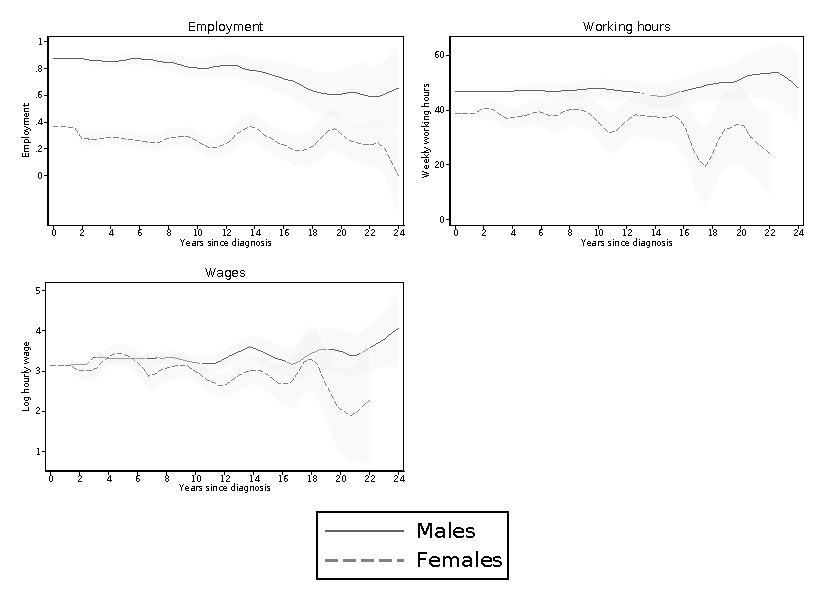
\includegraphics[width=\linewidth]{figures/lpoly_combined.pdf}\\
		\footnotesize{\textit{Notes} The shaded areas indicate the 95\% confidence intervals.}
	\end{center}
\end{figure}


Table \ref{tab:Self-reported-diabetes-duration} panel A shows the results of estimating Eq \ref{eq:duration_linear}, which indicated that male and female employment probabilities fell every year, with a larger effect shown by the within coefficient. \begin{table}[!ht]
	\caption{\label{tab:Self-reported-diabetes-duration}{\bf Relationship between self-reported years since diagnosis and employment probabilities using continuous duration and duration splines.}}
	\begin{center}
		%\resizebox{\linewidth}{!}{%
		\begin{adjustbox}{max width=.9\linewidth}
			\begin{threeparttable}
				{
					\def\sym#1{\ifmmode^{#1}\else\(^{#1}\)\fi}
					\begin{tabular}{l*{6}{S S}}
						\toprule
						&\multicolumn{2}{c}{Employment}       &\multicolumn{2}{c}{Weekly work hours}&\multicolumn{2}{c}{Log hourly wages} \\\cmidrule(lr){2-3}\cmidrule(lr){4-5}\cmidrule(lr){6-7}
						&\multicolumn{1}{c}{Males}&\multicolumn{1}{c}{Females}&\multicolumn{1}{c}{Males}&\multicolumn{1}{c}{Females}&\multicolumn{1}{c}{Males}&\multicolumn{1}{c}{Females}\\
						\midrule
						\textit{\textbf{Panel A: linear effect}} &&&&&&\\
						Years since diagnosis (within)&   -0.016\sym{***}&   -0.009\sym{*}  &    0.185         &    0.115         &   -0.016         &   -0.067\sym{**} \\
						&  (0.006)         &  (0.005)         &  (0.334)         &  (0.652)         &  (0.018)         &  (0.029)         \\
						Years since diagnosis (between)&   -0.008\sym{***}&   -0.005\sym{***}&   -0.021         &   -0.140         &    0.010\sym{**} &   -0.010         \\
						&  (0.002)         &  (0.001)         &  (0.107)         &  (0.125)         &  (0.005)         &  (0.009)         \\
						Within=Between (p-value)&    0.139         &    0.482         &    0.560         &    0.696         &    0.165         &    0.061         \\
						\textit{\textbf{Panel B: splines}} &&&&&&\\
						Years since SR diagnosis  &&&&&&\\
						Within effects&                  &                  &                  &                  &                  &                  \\
						0--3 &    -0.013         &   -0.018         &    0.708         &    2.953         &   -0.005         &    0.047         \\
						&  (0.014)         &  (0.016)         &  (0.857)         &  (2.700)         &  (0.054)         &  (0.124)         \\
						4--7 &    -0.011         &   -0.002         &    0.215         &   -2.517         &   -0.032         &   -0.131         \\
						&  (0.014)         &  (0.014)         &  (0.761)         &  (1.752)         &  (0.046)         &  (0.101)         \\
						8--12 &    0.003         &   -0.003         &   -1.153         &    1.144         &   -0.009         &   -0.053         \\
						&  (0.021)         &  (0.014)         &  (1.252)         &  (1.635)         &  (0.065)         &  (0.061)         \\
						13+ &    -0.039\sym{***}&   -0.015         &    0.720         &    0.184         &   -0.007         &   -0.096\sym{***}\\
						&  (0.014)         &  (0.010)         &  (0.943)         &  (1.414)         &  (0.057)         &  (0.037)         \\
						Between effects&                  &                  &                  &                  &                  &                  \\
						0--3 &    0.005         &    0.010         &   -0.030         &    0.204         &    0.042\sym{**} &    0.032         \\
						&  (0.008)         &  (0.009)         &  (0.465)         &  (0.653)         &  (0.020)         &  (0.032)         \\
						4--7 &    -0.003         &   -0.034         &   -0.444         &    0.727         &   -0.025         &   -0.034         \\
						&  (0.021)         &  (0.023)         &  (1.195)         &  (1.471)         &  (0.052)         &  (0.065)         \\
						8--12 &   -0.055\sym{**} &    0.004         &    1.110         &   -1.525         &   -0.031         &   -0.109         \\
						&  (0.023)         &  (0.024)         &  (1.367)         &  (1.647)         &  (0.060)         &  (0.075)         \\
						13+ &    0.004         &   -0.004         &   -0.432         &   -0.282         &    0.034\sym{*}  &    0.015         \\
						&  (0.008)         &  (0.003)         &  (0.476)         &  (0.245)         &  (0.019)         &  (0.017)         \\
						Within=Between (p-value)&  0.028         &    0.404         &    0.507         &    0.597         &    0.781         &    0.083         \\
						\textit{\textbf{Panel C: dummies}} &&&&&&\\
						within effects&                  &                  &                  &                  &                  &                  \\
						0--3&    0.005         &   -0.007         &    0.352         &   17.309\sym{*}  &    0.223         &   -0.447         \\
						&  (0.052)         &  (0.059)         &  (3.123)         &  (9.975)         &  (0.186)         &  (0.549)         \\
						4--7&    -0.031         &   -0.049         &    2.860         &   10.878         &    0.047         &   -0.568         \\
						&  (0.042)         &  (0.050)         &  (2.664)         &  (9.504)         &  (0.127)         &  (0.544)         \\
						8--12&    -0.066         &   -0.026         &   -0.709         &   13.733         &   -0.133         &   -0.873\sym{*}  \\
						&  (0.063)         &  (0.059)         &  (4.181)         &  (9.695)         &  (0.207)         &  (0.521)         \\
						13+&   -0.134         &   -0.062         &   -3.379         &   13.309         &    0.164         &   -0.882\sym{**} \\
						&  (0.098)         &  (0.068)         &  (4.715)         &  (9.239)         &  (0.284)         &  (0.446)         \\
						Between effects&                  &                  &                  &                  &                  &                  \\
						0--3&      -0.002         &    0.033         &   -0.760         &    0.322         &    0.109\sym{*}  &    0.023         \\
						&  (0.027)         &  (0.026)         &  (1.370)         &  (1.944)         &  (0.057)         &  (0.091)         \\
						4--7&    0.036         &    0.016         &   -1.004         &    3.157         &    0.154\sym{**} &    0.082         \\
						&  (0.030)         &  (0.042)         &  (1.968)         &  (3.208)         &  (0.076)         &  (0.134)         \\
						8--12&  -0.128\sym{**} &   -0.199\sym{***}&    2.231         &   -0.792         &   -0.069         &   -0.197         \\
						&  (0.065)         &  (0.055)         &  (3.111)         &  (4.043)         &  (0.131)         &  (0.161)         \\
						13+&   -0.187\sym{***}&   -0.076\sym{*}  &   -1.443         &   -4.127         &    0.196         &   -0.342\sym{**} \\
						&  (0.050)         &  (0.042)         &  (2.895)         &  (3.492)         &  (0.142)         &  (0.173)         \\
						Within=Between (p-value)&  0.397         &    0.060         &    0.672         &    0.242         &    0.721         &    0.745         \\
						\midrule
						N         &    16298         &    22427         &    10771         &     5746         &    13583         &     7391         \\
						\bottomrule
					\end{tabular}
					\begin{tablenotes}
						\item \footnotesize \textit{Notes} Panel A presents the results of the linear specifications. Panel B presents the results of the non-linear specifications. Robust standard errors in parentheses. All models include variables for  states, urbanization, level of education, marital status, number of children < 6, wealth, health insurance status, age squared and one dummy variable for each calendar year. \sym{*} \(p<0.10\), \sym{**} \(p<0.05\), \sym{***} \(p<0.01\).
					\end{tablenotes}
				}
			\end{threeparttable}
		\end{adjustbox}
	\end{center}
\end{table}
For females, the within coefficient also suggested a reduction in wages as diabetes progressed while the between coefficient showed no association for women and a relatively small positive association with male wages. Using diabetes onset groups, there was no evidence of an effect of diabetes duration for early onset groups (see Supplementary Table \ref{tab:Self-reported-diabetes-duration_earlylate}). However, again the within results for early onset should be interpreted with caution due to the limited number of diabetes incidence cases in this group, which also prohibited the estimation of any within effects of early diabetes onset duration for wages and working hours. The results also indicated that the effects found in Table \ref{tab:Self-reported-diabetes-duration} were driven mainly by those with a diabetes onset after age 35.


The non-linear results for the spline function and dummy variable approach are  presented in panels B and C, respectively. They suggest that the main adverse effects appeared after a prolonged time of living with diabetes; i.e. after more than seven years since diagnosis. The same was true for female wages. The lack of a statistically significant effect for the earlier years of diabetes duration may have been due to a reduction in statistical efficiency, reduced by the separation into duration groups and into within and between variation. Re-estimating the specifications with a random effects model that combined both types of variation into one estimate showed that, at least for the models with dummies, there was a more or less immediate reduction in employment probabilities that became stronger the longer a person had diabetes (see Supplementary Table \ref{tab:Self-reported-diabetes-duration_RE}). Note that we did not estimate models splitting diabetes in early and late onset groups, as this implied strong reductions in statistical power.

\FloatBarrier

\subsection{Cross-sectional biomarker analysis}


As reported in Supplementary Table \ref{tab:Biomarker_observations}, 18\% of the observations in the biomarker sample were false negatives, i.e. undiagnosed. Further, 2\% were false positives, though the latter may have included cases that received a diabetes diagnosis and managed to reduce their \ac{HbA1c} to non-diabetes levels via medication and/or lifestyle changes \parencite{Flores-Hernandez2015}. Overall 80\% of the self-reports were consistent with the biomarker data. Comparing the health status and diabetes risk factors of the diagnosed and undiagnosed diabetes populations suggested that those with self-reported diabetes were older and in worse health, both objectively and subjectively compared to those undiagnosed. This suggests a selection into the diagnosed group based on the severity and potentially duration of diabetes. If the adverse effects of diabetes are due to its health impact, we would suspect worse labour market outcomes for the diagnosed compared to the undiagnosed population.


\begin{table}[!ht]
	\caption{\label{tab:Diagnosed_vs_undiagnosed}{\bf Descriptive comparison of diagnosed and undiagnosed population with diabetes.}}
	\begin{center}
		\begin{adjustbox}{max width=\linewidth}
			\begin{threeparttable}
				{
					\def\sym#1{\ifmmode^{#1}\else\(^{#1}\)\fi}
					\begin{tabular}{l*{6}{S S}}
						\toprule
						&\multicolumn{3}{c}{Males}             &\multicolumn{3}{c}{Females}\\\cmidrule(lr){2-4}\cmidrule(lr){5-7} 
						&\multicolumn{1}{c}{Diagnosed} &\multicolumn{1}{c}{Undiagnosed}&  \multicolumn{1}{c}{P value}&\multicolumn{1}{c}{Diagnosed}
						&\multicolumn{1}{c}{Undiagnosed} &\multicolumn{1}{c}{P value}\\
						&\multicolumn{1}{c}{diabetes} &\multicolumn{1}{c}{diabetes}&  \multicolumn{1}{c}{(t-test)}&\multicolumn{1}{c}{diabetes}&\multicolumn{1}{c}{diabetes}  &\multicolumn{1}{c}{(t-test)}\\
						\midrule
						Employed            &       0.807&       0.875&       0.012&       0.241&       0.331&       0.002\\
						Hourly wage         &      35.931&      30.670&       0.120&      36.092&      32.638&       0.550\\
						Usual weekly working hours&      44.341&      46.682&       0.104&      34.708&      39.681&       0.046\\
						Age                 &      53.162&      44.720&       0.000&      53.167&      44.449&       0.000\\
						Any medical insurance&       0.677&       0.599&       0.033&       0.733&       0.643&       0.002\\
						City of 2,5oo-15,000&       0.096&       0.107&       0.643&       0.112&       0.112&       0.994\\
						City of 15,000-100,000&       0.135&       0.096&       0.098&       0.087&       0.090&       0.884\\
						City of >100,000    &       0.331&       0.297&       0.325&       0.294&       0.333&       0.185\\
						Married             &       0.719&       0.643&       0.031&       0.633&       0.569&       0.035\\
						Number of children (age<6) in household&       0.950&       1.122&       0.073&       0.960&       1.257&       0.001\\
						Indigenous group    &       0.158&       0.211&       0.079&       0.195&       0.207&       0.626\\
						Primary             &       0.479&       0.434&       0.238&       0.626&       0.465&       0.000\\
						Secondary           &       0.212&       0.231&       0.554&       0.132&       0.233&       0.000\\
						High school         &       0.062&       0.131&       0.003&       0.037&       0.117&       0.000\\
						Higher education    &       0.139&       0.113&       0.288&       0.030&       0.073&       0.003\\
						Wealth index        &      -0.174&       0.117&       0.000&       0.012&       0.103&       0.157\\
						Subjective health       &&&&&&\\
						\hspace*{10mm}very good&       0.023&       0.094&       0.000&       0.012&       0.054&       0.001\\
						\hspace*{10mm}good     &       0.212&       0.434&       0.000&       0.180&       0.367&       0.000\\
						\hspace*{10mm}fair     &       0.619&       0.442&       0.000&       0.643&       0.528&       0.000\\
						\hspace*{10mm}bad      &       0.135&       0.026&       0.000&       0.155&       0.048&       0.000\\
						\hspace*{10mm}very bad &       0.012&       0.004&       0.187&       0.010&       0.004&       0.246\\
						Glycated hemoglobin (HbA1c)&       9.037&       8.533&       0.004&       8.979&       8.680&       0.049\\
						Hypertension (self-reported)       &       0.262&       0.074&       0.000&       0.397&       0.150&       0.000\\
						Blood pressure       &&&&&&\\
						\hspace*{10mm}Systolic             &     136.688&     130.506&       0.000&     136.070&     122.835&       0.000\\
						\hspace*{10mm}Diastolic            &      84.677&      82.063&       0.003&      84.495&      79.689&       0.000\\
						Heart disease (self-reported)      &       0.035&       0.007&       0.004&       0.050&       0.024&       0.021\\
						BMI     &      28.868&      28.311&       0.135&      30.640&      29.778&       0.032\\
						Obese (BMI $\geq 30$)&       0.338&       0.311&       0.440&       0.469&       0.431&       0.225\\
						\bottomrule
					\end{tabular}
					\begin{tablenotes}
						\item \footnotesize \textit{Notes} Mean values. \sym{*} \(p<0.10\), \sym{**} \(p<0.05\), \sym{***} \(p<0.01\).
					\end{tablenotes}
				}
			\end{threeparttable}
		\end{adjustbox}
	\end{center}
\end{table}


Table \ref{tab:Biomarker_results} presents the results from estimating Eq. \ref{eq:diab_sr} -- \ref{eq:diab_hba1c}. Panel A confirms the earlier longitudinal results using self-reported diabetes for the cross-sectional biomarker sample. The results in panel B indicate that the relationship with employment became weaker when using diabetes defined by the biomarker instead of self-reported diabetes, in particular for men. Results in Panel C were obtained from estimating Eq. \ref{eq:diab_ud} and indicate an absence of a (statistically significant) negative relationship between undiagnosed diabetes (expressed in the 'Biomarker diabetes but not self-reported' coefficient) and labour outcomes. The coefficients for the interaction term were mostly negative, though only statistically significant in the case of female working hours. 


\begin{table}[!ht]
	\caption{\label{tab:Biomarker_results}{\bf Biomarker results.}}
	\begin{center}
		\begin{adjustbox}{max width=\linewidth}
			\begin{threeparttable}
				{
					\def\sym#1{\ifmmode^{#1}\else\(^{#1}\)\fi}
					\begin{tabular}{l*{6}{S
								S}}
						\toprule
						&\multicolumn{2}{c}{Employment}       &\multicolumn{2}{c}{Weekly work hours}&\multicolumn{2}{c}{Log hourly wages} \\\cmidrule(lr){2-3}\cmidrule(lr){4-5}\cmidrule(lr){6-7}
						&\multicolumn{1}{c}{Males}&\multicolumn{1}{c}{Females}&\multicolumn{1}{c}{Males}&\multicolumn{1}{c}{Females}&\multicolumn{1}{c}{Males}&\multicolumn{1}{c}{Females}\\
						\midrule
						\multicolumn{7}{l}{\textbf{Panel A: Diabetes (self-reported)}} \\ 
				
						Self-reported diabetes&   -.055\sym{**} &    -.050\sym{**} &    -.308         &    -.323         &    -.026         &    -.005         \\
						&   (.026)         &   (.024)         &  (1.321)         &  (2.190)         &   (.066)         &   (.105)         \\
						\multicolumn{7}{l}{\textbf{Panel B: Diabetes (biomarker)}} \\
						Biomarker diabetes (HbA1c $\geq 6.5$)&    -.012         &    -.032\sym{*}  &    -.060         &    1.067         &    -.008         &    -.041         \\
						&   (.016)         &   (.018)         &   (.844)         &  (1.470)         &   (.045)         &   (.071)         \\
						\multicolumn{7}{l}{\textbf{Panel C: Interacting self-reported and biomarker diabetes}} \\
						Self-reported diabetes but tested negative ($\beta_{1}$)& -.049         &    -.027         &    1.547         &    7.417         &     .250         &    -.025         \\
						&   (.059)         &   (.051)         &  (3.446)         &  (4.669)         &   (.205)         &   (.232)         \\
						Biomarker diabetes but not self-reported (HbA1c $\geq 6.5$) ($\beta_{2}$)&     .005         &    -.020         &     .174         &    2.304         &     .015         &    -.049         \\
						&   (.018)         &   (.020)         &   (.960)         &  (1.639)         &   (.050)         &   (.078)         \\
						Self-reported diabetes and biomarker diabetes ($\beta_{3}$) &    -.011         &    -.015         &   -2.255         &  -11.484\sym{**} &    -.319         &     .059         \\
						&   (.065)         &   (.059)         &  (3.772)         &  (5.423)         &   (.220)         &   (.265)         \\
						All self-reported ($\beta_{1}+\beta_{3}$)&   -.060\sym{**}        &    -.042         &    -.708         &   -4.067         &    -.069         &     .034         \\
						&   (.029)         &   (.031)         &  (1.571)         &  (2.813)         &   (.084)         &   (.137)         \\ 
						\multicolumn{7}{l}{\textbf{Panel D: HbA1c levels}} \\ 
						Self-reported diabetes&  -.067         &    -.035         &    1.471         &    4.974         &     .157         &    -.017         \\
						&   (.072)         &   (.041)         &  (2.619)         &  (3.654)         &   (.119)         &   (.186)         \\
						HbA1c if $\geq 6.5$  &    .001         &    -.003         &    -.005         &     .235         &     .002         &    -.005         \\
						&   (.002)         &   (.002)         &   (.104)         &   (.193)         &   (.005)         &   (.008)         \\
						Self-reported diabetes $\times$ HbA1c if $\geq 6.5$&    .001         &     .000         &    -.207         &    -.852\sym{**} &    -.023         &     .005         \\
						&   (.007)         &   (.005)         &   (.294)         &   (.424)         &   (.014)         &   (.022)         \\
						\midrule                 
						N               &\multicolumn{1}{c}{2785}         &\multicolumn{1}{c}{3620}         &\multicolumn{1}{c}{2302}         &\multicolumn{1}{c}{1142}         &\multicolumn{1}{c}{1803}         &\multicolumn{1}{c}{882}         \\
						\bottomrule
					\end{tabular}
					\begin{tablenotes}
						\item \footnotesize \textit{Notes} Results are based on community level fixed effects. Robust standard errors in parentheses. All models include variables for  states, urbanization, level of education, marital status, number of children < 6, wealth, health insurance status, age squared and one dummy variable for each calendar year to account for the multiple years of data collection for the third wave. The wage and working hour models additionally control for type of work (agricultural and self employed with non-agricultural wage employment as the base). \sym{*} \(p<0.10\), \sym{**} \(p<0.05\), \sym{***} \(p<0.01\).
					\end{tablenotes}
				}
			\end{threeparttable}
		\end{adjustbox}
	\end{center}
\end{table}


To explore whether the adverse effects increased with higher  \ac{HbA1c} levels, we estimated Eq. \ref{eq:diab_hba1c}. The results in panel D again only suggest a negative association of a one percentage point increase in \ac{HbA1c} with female working hours for those with self-reported diabetes. For undiagnosed diabetes, we again found no effects.

\FloatBarrier
	
\section{\label{sec:cha_4_conclusion}Discussion}

Diabetes is now one of the most common chronic diseases in low- and middle income countries, as well as high-income countries, with potential severe impacts on the health and economic well-being of those affected.  Yet rigorous evidence on the economic consequences for \acp{LMIC} remains scarce.

To address key methodological challenges, this paper used rich longitudinal panel data from Mexico that also contained diabetes biomarkers. The biomarker data showed alarming levels of clinically tested diabetes (27\% prevalence) and indicate that a large proportion of the Mexican population (18\%) is unaware of their condition.

Overall, the paper found evidence for adverse effects of self-reported diabetes on the probability of being employed, confirming earlier findings for Mexico that used cross-sectional information. But, these new results also suggest a comparatively larger impact of diabetes on female employment probabilities. The evidence also points towards the main effects being driven by those with a diabetes onset at a relatively later state, consisting most likely of people with type 2 diabetes. Analyses of the long term impact indicated that the employment probability fell gradually in the years following diagnosis. The results for the non-linear models were less clear, potentially due to reductions in statistical power, but suggest that adverse effects became stronger with time since diagnosis. The linear effect contrasts with estimates for the USA, where such an effect seemed to be absent, however allowing for non-linearity revealed falling employment probabilities after 11 to 15 years for females and after 2-5 years for males \parencite{Minor2013}. For working hours and wages, our results were more ambiguous with adverse effects being observed for time since diagnosis on female wages only. In summary, most of the adverse effects of diabetes were found at the extensive margin, mainly affecting the probability of employment, rather than the intensive margin, i.e. working hours or wages. 

Overall, a relationship of diabetes with working hours or wages is mostly absent, except for the between estimator in the case of wages for men. Contrasting the between and within results suggests that this significant result may have arisen from individual selection. Although any explanation at this point is speculative, it may be that higher paid men, who also tend to be more educated, were able to remain employed without experiencing wage reductions, for instance due to their particular set of skills. They may also have had access to better health care leading to better diabetes related health outcomes. Low paid workers, on the other hand, may lack access to quality diabetes care, making it more likely that they develop severe complications earlier \parencite{Flores-Hernandez2015}. They are also more likely to be in informal employment and low skilled jobs, with less job security and are thus more prone to being laid off to be replaced with healthier workers.

Because self-reported diabetes may not adequately represent the entire diabetes population if the share of undiagnosed diabetes is relatively large and those undiagnosed differ from those diagnosed, estimates based on self-reported diabetes are likely to be biased. Our results using the cross-sectional biomarker data suggest indeed that  those with undiagnosed diabetes were significantly healthier and younger. Consequently, diabetes based on biomarkers was found to be less related to reduced employment, compared to self-reported diabetes, in particular for men. Further analysis showed that this was due to the absence of any association between undiagnosed diabetes and employment. These results are similar to those found for the USA, where no statistically significant relationship was observed between undiagnosed diabetes on employment, while a significant effect of diagnosed diabetes was observed \parencite{Minor2015}. Our results further indicate that the  difference in the employment effects of diagnosed and undiagnosed diabetes was not mediated by current \ac{HbA1c} levels, similar to findings for Mexican-Americans in the USA, where employment outcomes were unrelated to higher \ac{HbA1c} levels \parencite{BrownIII2011}. This may stem from \ac{HbA1c} levels primarily being informative for the last three months, and not being the only indicator for the severity of diabetes. Overall, it seems that general health differences related to a longer diabetes duration and selection into the diagnosed population, for instance based on emerging diabetes related health problems, could be driving the adverse economic effects among those with a self-reported diagnosis.

Our study had several limitations. While the within-coefficient accounts for any time-invariant confounding, the estimates may have been affected by unobserved time-variant confounders. Reverse causality, where employment status affects the propensity to develop or be diagnosed with diabetes, may also play a role. Existing studies that looked at this particular direction of causality, however, have not found strong evidence for an effect of employment status on diabetes \parencite{Bergemann2011,Schaller2015}, though they were carried out in high-income countries. For the duration analysis an additional limitation, imposed by the data, was that the year of diagnosis was only reported in the third wave. While this still allowed us to construct an estimate of the time since diagnosis for the previous waves, it restricted the analysis to those that were present in the last wave, thereby excluding those that dropped out of the sample prior to the third wave. 

Despite these limitations, our findings bear important implications. First, the impact of self-reported diabetes on labor outcomes in Mexico seems mostly limited to its effect on employment probabilities, though there is some indication that it could also reduce wages over time for women.  Second, its effect on employment was much stronger for females, though the underlying reasons for this remain unclear. Potential explanations are that lower working hours or wages for women make dropout less costly. Other evidence suggests that women with diabetes are in worse metabolic health compared to men when they cross the diabetes threshold \parencite{Peters2015}, making it more likely for them to drop out. Third, caution is needed when estimates based on self-reported diabetes are interpreted in terms of the entire population, i.e. extending to those with undiagnosed diabetes. Ideally, studies would  include a biomarker analysis, acknowledge the differences between diagnosed and undiagnosed subpopulations, and carry out a separate analysis whenever feasible. If this is not possible, study conclusions about the effect of self-reported diabetes should be limited to this specific part of the population, in particular in environments where the share of undiagnosed diabetes is high, as is the case for most low- and middle income countries.

While we find no effect for undiagnosed diabetes in our cross section analysis, further inquiry over time is needed. The large proportion of previously undiagnosed cases indicates that diagnosis—at least in Mexico—happens late or not at all. This may reduce the possibilities to prevent complications via treatment and self-management, increasing the risk of severe complications appearing premature. Earlier diagnosis and ensuing effective treatment may lighten the health and economic burden. Further analysis is also needed to explain why the adverse economic effects are so large for women. Ultimately, prevention of diabetes is of high importance. Taxation of sugar sweetened beverages may be one promising way forward \parencite{Colchero2016}, though their long-term effectiveness remains unclear. Given the established links between early life heath and later life incidence of diabetes as well as other chronic diseases \parencite{Sotomayor2013,Hanson2012,Li2010b}, investments in maternal and child health may be particularly attractive to address non-communicable and communicable diseases at the same time.

\printbibliography


	
\clearpage
\setcounter{table}{0}
\renewcommand{\thetable}{S\arabic{table}}
\setcounter{figure}{0}
\setcounter{page}{1}
\renewcommand{\thefigure}{S\arabic{figure}} %changes chapter number to roman
\section*{Supplementary material}

\subsection*{\label{sec:Appendix}Strategies to deal with inconsistent self-reporting over time}

Reporting error can pose a considerable challenge in the use of self-reported data. Fortunately, the \ac{MxFLS} data provide several possibilities to assess the amount of misreporting and apply corrections before estimating the labour market effects of diabetes. In what follows we describe how we have dealt with inconsistencies in self-reported diabetes over time.

Throughout the surveys, self-reported diabetes was measured by the question 'Have you ever been diagnosed by diabetes'. One of the key advantages of panel data is the repeated measurement which results in more than one data point, allowing to uncover inconsistencies for cases with multiple observations. Very little is known about inconsistencies in self-reported diabetes over time. \textcite{Zajacova2010} assess the consistency of a self-reported cancer diagnosis over time in the USA. The study found that 30\% of those who had reported a cancer diagnosis at an earlier point failed to report the diagnosis at a later point in time. A more recent diagnosis was found to be reported with greater consistency possibly due to increasing recall problems as time since diagnosis advanced.

When assessing the \ac{MxFLS}, we also found inconsistencies in the diabetes self-reports across the three waves, with between 10--20\% of those reporting diabetes in one wave not doing so in one of the subsequent waves. To improve the validity of diabetes self-reports, we were interested in reducing the amount of reporting inconsistencies.

For diabetes, the main concern with mismeasurement is related to false negatives. False positives are deemed less of a problem since incentives to report diabetes when one does not have it seem to be very limited---although we cannot exclude this.  A study from China finds that the vast majority (98\%) of those who self-report diabetes are tested positive for diabetes, while only a minority  of those who are tested positive for diabetes (40\%) actually self-report the disease \parencite{Yuan2015}.  Our data showed a similar pattern, with a low proportion (3\%) of the respondents being tested negative while self-reporting diabetes, while the majority of those who are tested positive (68\%) do not self-report diabetes.

We used the above information to infer the "true" diabetes status for those with inconsistent reports. For respondents present in all three waves, we corrected inconsistencies as reported in Supplementary Table \ref{tab:Inconsistencies}. We assumed that if diabetes was reported only once in the first two waves (either in 2002 or 2005) and then not reported again in the ensuing waves, this diabetes report was likely to be false (see lines 3 and 4 in Supplementary Table \ref{tab:Inconsistencies}) and that the person never had received a diagnosis. If a diabetes diagnosis was however reported in two of the three waves (in 2002 and 2009 but not 2005, or in 2002 and 2005 but not in 2009) we assumed that the respondent had diabetes in all three waves (see lines 1 and 2 in Supplementary Table \ref{tab:Inconsistencies}). For cases where we only had information from two waves, we assumed that if a diabetes diagnosis had been reported in a prior wave they also had diabetes in the ensuing wave, even if it was not reported in the latter (see lines 5 and 6 in Supplementary Table \ref{tab:Inconsistencies}), given that most diabetes self-reports tend to be correct.

\begin{table}[!ht]
	\caption{\label{tab:Inconsistencies}Inconsistencies in diabetes self-report in MxFLS.}
	\begin{center}
		\begin{adjustbox}{max width=\linewidth} 
			\begin{tabular}{lllc}
				\hline 
				&Inconsistency  & Assumption  & Number of observations replaced\tabularnewline
				\hline 
				1 &Diabetes self-report only in 2002, but not in 2005 and 2009  & Has no diabetes in 2002 either  & 66\tabularnewline
				2 &Diabetes self-report only in 2005, but not in 2002 and 2009  & Has no diabetes in 2005 either  & 52\tabularnewline
				3 &Diabetes self-report in 2002, 2005 but not in 2009  & Has diabetes in 2009 as well  & 19\tabularnewline
				4 &Diabetes self-report in 2002, 2009 but not in 2005  & Has diabetes in 2005 as well  & 63\tabularnewline
				5 &Diabetes self-report in 2002, but not in 2005. Not in survey in 2009  & Has diabetes in 2005 as well  & 44\tabularnewline
				6 &Diabetes self-report in 2005, but not in 2009. Not in survey in 2002  & Has diabetes in 2009 as well  & 23\tabularnewline
				\hline 
			\end{tabular}
		\end{adjustbox}
	\end{center}
\end{table}

We then tested if those respondents we categorized as not having a diabetes diagnosis based on above rules were actually more likely to not have biometrically measured diabetes, using the biomarker data from wave 3. Of those with inconsistencies in their diabetes self-reports, 95 were present in the biomarker sample (46 with two self-reports (from lines 3 and 4 in Table \ref{tab:Inconsistencies}) and 49 with one self-report of diabetes (from lines 1 and 2 in Supplementary Table \ref{tab:Inconsistencies})). Supplementary Figure \ref{fig:kdens_inconsistency_hba1c} illustrates the difference between both groups and suggests that indeed those with two self-reports of diabetes are much more likely to have \ac{HbA1c} values above the diabetes threshold. A t-test comparing the mean \ac{HbA1c} for the two groups indicates that those with two self-reports also have significantly (p<0.001) higher \ac{HbA1c} levels than those with only one self-report of diabetes (9.7\% vs. 7.1\%). Further, of those with one self-report,  only 30\% have an \ac{HbA1c}$\geq6.5$\% compared to 87\% of those with two self-reports. Based on these results it appears that we did minimize misclassification of people into diabetes or no-diabetes. 

\begin{figure}[h!]
	\caption{\label{fig:kdens_inconsistency_hba1c}Kernel density of HbA1c values for those with one inconsistent and two inconsistent reports.}%
	\begin{center}
		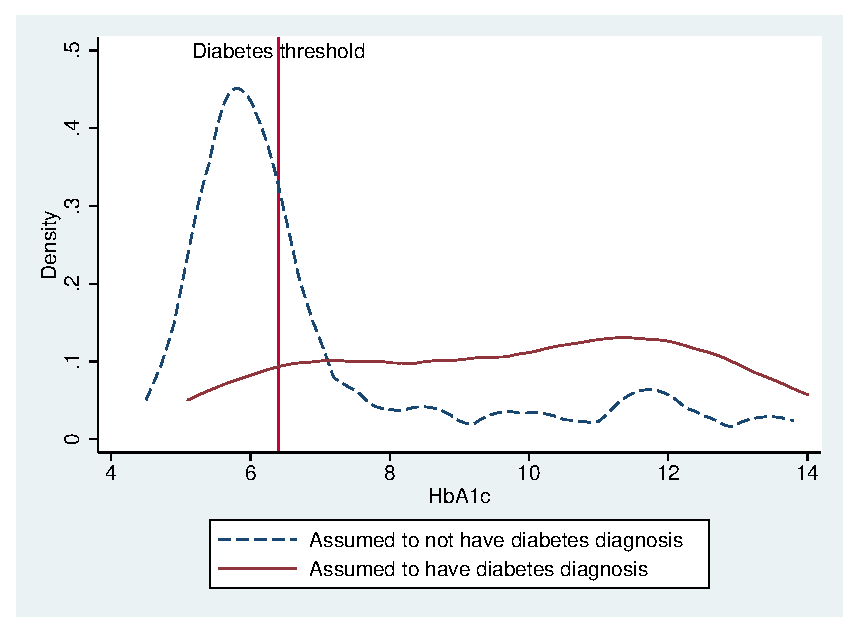
\includegraphics[width=.7\linewidth]{figures/kdensity_hba1c_inconsist.eps}\\
	\end{center}
\end{figure}


\clearpage

\subsection*{Early versus late onset of diabetes}

\begin{table}[!ht]
	\caption{\label{tab:Labour_outcomes_earlylate}{\bf Labour outcomes and self-reported diabetes by diabetes onset.}}
	\begin{center}
		\begin{adjustbox}{max width=\linewidth} 
			\begin{threeparttable} 
				{
					\def\sym#1{\ifmmode^{#1}\else\(^{#1}\)\fi}
					\begin{tabular}{l*{6}{S S}}
						\toprule
						&\multicolumn{2}{c}{Employment}    &\multicolumn{2}{c}{Weekly work hours} &\multicolumn{2}{c}{Log hourly wages}  \\\cmidrule(lr){2-3}\cmidrule(lr){4-5}\cmidrule(lr){6-7}
						&\multicolumn{1}{c}{Males}&\multicolumn{1}{c}{Females}&\multicolumn{1}{c}{Males}&\multicolumn{1}{c}{Females}&\multicolumn{1}{c}{Males}&\multicolumn{1}{c}{Females}\\
						\midrule
						Early onset (within)&    0.133         &   -0.206\sym{**} &   14.712\sym{*}  &  -18.636\sym{*}  &   -0.523         &    0.388\sym{***}\\
						&  (0.176)         &  (0.086)         &  (8.370)         &  (9.668)         &  (0.340)         &  (0.057)         \\
						Late onset (within)&   -0.059\sym{**} &   -0.048\sym{*}  &   -1.008         &   -1.322         &    0.079         &    0.067         \\
						&  (0.025)         &  (0.025)         &  (1.513)         &  (2.553)         &  (0.067)         &  (0.163)         \\
						Early onset (between)&    0.016         &   -0.052         &    1.483         &   -2.640         &   -0.102         &    0.286         \\
						&  (0.037)         &  (0.047)         &  (2.581)         &  (4.034)         &  (0.099)         &  (0.232)         \\
						Late onset (between)&   -0.087\sym{***}&   -0.067\sym{***}&   -1.077         &   -0.869         &    0.121\sym{**} &   -0.111\sym{*}  \\
						&  (0.017)         &  (0.016)         &  (0.895)         &  (1.375)         &  (0.050)         &  (0.066)         \\
						\midrule
						N         &    21388         &    27339         &    13828         &     7068         &    17616         &     9112         \\
						\bottomrule
					\end{tabular}
					\begin{tablenotes}
						\item \footnotesize \textit{Notes} Robust standard errors in parentheses. All models include variables for  states, urbanization, level of education, marital status, number of children < 6, wealth, health insurance status, age squared and one dummy variable for each calendar year. \sym{*} \(p<0.10\), \sym{**} \(p<0.05\), \sym{***} \(p<0.01\).
					\end{tablenotes}
				}
			\end{threeparttable}
		\end{adjustbox}
	\end{center}
\end{table} 
\clearpage

\begin{table}[p]
	\caption{\label{tab:Worktype_earlylate}{\bf Selection into types of work and self-reported diabetes by diabetes onset.}}
	\begin{center}
		\begin{adjustbox}{max width=\linewidth} 
			\begin{threeparttable} 
				{
					\def\sym#1{\ifmmode^{#1}\else\(^{#1}\)\fi}
					\begin{tabular}{l*{6}{S S}}
						\toprule
						&\multicolumn{2}{c}{Non-agric.}       &\multicolumn{2}{c}{Agriculture}      &\multicolumn{2}{c}{Self-employed}    \\\cmidrule(lr){2-3}\cmidrule(lr){4-5}\cmidrule(lr){6-7}
						&\multicolumn{1}{c}{Males}&\multicolumn{1}{c}{Females}&\multicolumn{1}{c}{Males}&\multicolumn{1}{c}{Females}&\multicolumn{1}{c}{Males}&\multicolumn{1}{c}{Females}\\
						\midrule
						Early onset (within)&     0.030         &   -0.105         &   -0.225         &   -0.068         &    0.328\sym{**} &   -0.027         \\
						&  (0.216)         &  (0.074)         &  (0.139)         &  (0.047)         &  (0.161)         &  (0.048)         \\
						Late onset (within)&  -0.008         &    0.007         &   -0.002         &   -0.019\sym{**} &   -0.053\sym{**} &   -0.030         \\
						&  (0.029)         &  (0.018)         &  (0.022)         &  (0.009)         &  (0.026)         &  (0.019)         \\
						Early onset (between)&     0.011         &   -0.050         &   -0.078\sym{***}&   -0.006         &    0.087         &    0.005         \\
						&  (0.055)         &  (0.043)         &  (0.030)         &  (0.007)         &  (0.056)         &  (0.029)         \\
						Late onset (between)&   -0.037\sym{*}  &   -0.048\sym{***}&   -0.091\sym{***}&   -0.009\sym{***}&    0.039\sym{*}  &   -0.014         \\
						&  (0.022)         &  (0.012)         &  (0.015)         &  (0.003)         &  (0.020)         &  (0.011)         \\
						\midrule
						N         &    20719         &    26575         &    20719         &    26575         &    20719         &    26575         \\
						\bottomrule
					\end{tabular}
					\begin{tablenotes}
						\item \footnotesize \textit{Notes} Robust standard errors in parentheses. All models include variables for  states, urbanization, level of education, marital status, number of children < 6, wealth, health insurance status, age squared and one dummy variable for each calendar year. \sym{*} \(p<0.10\), \sym{**} \(p<0.05\), \sym{***} \(p<0.01\).
					\end{tablenotes}
				}
			\end{threeparttable}
		\end{adjustbox}
	\end{center}
\end{table} 

\clearpage

\begin{table}[p]
	\caption{\label{tab:Self-reported-diabetes-duration_earlylate}{\bf Relationship between self-reported years since diagnosis and employment probabilities using continuous duration by diabetes onset.}}
	\begin{center}
		%\resizebox{\linewidth}{!}{%
		\begin{adjustbox}{max width=\linewidth}
			\begin{threeparttable}
				{
					\def\sym#1{\ifmmode^{#1}\else\(^{#1}\)\fi}
					\begin{tabular}{l*{6}{S S}}
						\toprule
						&\multicolumn{2}{c}{Employment}       &\multicolumn{2}{c}{Monthly work hours} &\multicolumn{2}{c}{Log hourly wages} \\\cmidrule(lr){2-3}\cmidrule(lr){4-5}\cmidrule(lr){6-7}
						&\multicolumn{1}{c}{Males}&\multicolumn{1}{c}{Females}&\multicolumn{1}{c}{Males}&\multicolumn{1}{c}{Females}&\multicolumn{1}{c}{Males}&\multicolumn{1}{c}{Females}\\
						\midrule
						Early onset (within)&   -0.009         &    0.002         &                  &                  &                  &                  \\
						&  (0.017)         &  (0.013)         &                  &                  &                  &                  \\
						Late onset (within)&   -0.012\sym{**} &   -0.007\sym{*}  &    0.086         &    0.308         &   -0.006         &   -0.059\sym{***}\\
						&  (0.005)         &  (0.004)         &  (0.275)         &  (0.504)         &  (0.013)         &  (0.022)         \\
						Early onset (between)&    0.011\sym{***}&   -0.016\sym{***}&   -0.016         &    0.029         &    0.187         &   -0.401         \\
						&  (0.004)         &  (0.005)         &    (0.012)         &  (0.051)         &  (0.333)         &  (0.896)         \\
						Late onset (between)&  -0.009\sym{***}&   -0.005\sym{***}&   -0.060         &   -0.144         &    0.011\sym{**} &   -0.010         \\
						&  (0.002)         &  (0.002)         &  (0.117)         &  (0.129)         &  (0.006)         &  (0.009)         \\
						\midrule
						N         &    16308         &    22450         &    13592         &     7394         &    10778         &     5748         \\
						\bottomrule
					\end{tabular}
					\begin{tablenotes}
						\item \footnotesize \textit{Notes} The within estimator for the effects of early onset diabetes on wages and working hours could not be estimates due to no within-variation for diabetes. Robust standard errors in parentheses. All models include variables for  states, urbanization, level of education, marital status, number of children < 6, wealth, health insurance status, age squared and one dummy variable for each calendar year. \sym{*} \(p<0.10\), \sym{**} \(p<0.05\), \sym{***} \(p<0.01\).
					\end{tablenotes}
				}
			\end{threeparttable}
		\end{adjustbox}
	\end{center}
\end{table}

\clearpage

\subsection*{Random effects model}

\begin{table}[!ht]
	\caption{\label{tab:Self-reported-diabetes-duration_RE}{\bf Relationship between self-reported years since diagnosis and employment probabilities using continuous duration and duration splines (random effects).}}
	\begin{center}
		%\resizebox{\linewidth}{!}{%
		\begin{adjustbox}{max width=\linewidth}
			\begin{threeparttable}
				{
					\def\sym#1{\ifmmode^{#1}\else\(^{#1}\)\fi}
					\begin{tabular}{l*{6}{S S}}
						\toprule
						&\multicolumn{2}{c}{Employment}       &\multicolumn{2}{c}{Weekly work hours}&\multicolumn{2}{c}{Log hourly wages} \\\cmidrule(lr){2-3}\cmidrule(lr){4-5}\cmidrule(lr){6-7}
						&\multicolumn{1}{c}{Males}&\multicolumn{1}{c}{Females}&\multicolumn{1}{c}{Males}&\multicolumn{1}{c}{Females}&\multicolumn{1}{c}{Males}&\multicolumn{1}{c}{Females}\\
						\midrule
						\textit{\textbf{Panel A: linear effect}} &&&&&&\\
						Years since diagnosis&  -0.007\sym{***}&   -0.004\sym{***}&    0.039         &   -0.130         &    0.010\sym{**} &   -0.009         \\
						&  (0.002)         &  (0.001)         &  (0.102)         &  (0.127)         &  (0.005)         &  (0.008)         \\
						\textit{\textbf{Panel B: splines}} &&&&&&\\
						Years since SR diagnosis  &&&&&&\\              &                  &                  &                  &                  &                  \\
						0--3 &     -0.008         &   -0.015\sym{**} &   -0.035         &    0.507         &    0.038\sym{**} &    0.034         \\
						&  (0.006)         &  (0.006)         &  (0.346)         &  (0.614)         &  (0.017)         &  (0.029)         \\
						4--7   &    0.001         &    0.004         &    0.242         &   -0.570         &   -0.032         &   -0.048         \\
						&  (0.011)         &  (0.011)         &  (0.665)         &  (1.062)         &  (0.032)         &  (0.052)         \\
						8--12   &   -0.008         &    0.002         &   -0.116         &   -0.080         &   -0.003         &   -0.074         \\
						&  (0.015)         &  (0.011)         &  (0.855)         &  (1.098)         &  (0.041)         &  (0.050)         \\
						13+   &    -0.012         &   -0.004         &    0.035         &   -0.339         &    0.029         &    0.011         \\
						&  (0.008)         &  (0.003)         &  (0.410)         &  (0.241)         &  (0.018)         &  (0.017)         \\
						\textit{\textbf{Panel C: dummies}} &&&&&&\\
						0--3&   -0.036\sym{*}  &   -0.041\sym{**} &   -0.821         &    1.091         &    0.134\sym{**} &    0.021         \\
						&  (0.021)         &  (0.021)         &  (1.154)         &  (1.826)         &  (0.054)         &  (0.083)         \\
						4--7&   -0.014         &   -0.056\sym{**} &    0.877         &    1.200         &    0.093         &   -0.003         \\
						&  (0.022)         &  (0.023)         &  (1.375)         &  (2.530)         &  (0.059)         &  (0.118)         \\
						8--12 &  -0.069\sym{*}  &   -0.043         &    0.427         &    0.302         &   -0.070         &   -0.148         \\
						&  (0.037)         &  (0.030)         &  (2.288)         &  (2.995)         &  (0.101)         &  (0.117)         \\
						13+ &   -0.121\sym{***}&   -0.043         &   -0.568         &   -2.104         &    0.242\sym{*}  &   -0.279\sym{*}  \\
						&  (0.045)         &  (0.031)         &  (2.280)         &  (3.088)         &  (0.126)         &  (0.153)         \\
						\midrule
						N         &    16308         &    22450         &    13592         &     7394         &    10778         &     5748         \\
						\bottomrule
					\end{tabular}
					\begin{tablenotes}
						\item \footnotesize \textit{Notes} Panel A presents the results of the linear specifications. Panel B presents the results of the non-linear specifications. Robust standard errors in parentheses. All models include variables for  states, urbanization, level of education, marital status, number of children < 6, wealth, health insurance status, age squared and one dummy variable for each calendar year. \sym{*} \(p<0.10\), \sym{**} \(p<0.05\), \sym{***} \(p<0.01\).
					\end{tablenotes}
				}
			\end{threeparttable}
		\end{adjustbox}
	\end{center}
\end{table}

\clearpage

\begin{table}[!ht]
	\caption{\label{tab:Biomarker_observations}{\bf Number of observations with diabetes (HbA1c $\geq 6.5\%$) and self-reported diabetes.}}
	\begin{center}
		\begin{adjustbox}{max width=\linewidth}
			\begin{threeparttable}
				{
					\def\sym#1{\ifmmode^{#1}\else\(^{#1}\)\fi}
					\begin{tabular}{lcccc}
						\toprule
						&\multicolumn{1}{c}{$HbA1c < 6.5\%$}&\multicolumn{1}{c}{HbA1c $\geq 6.5\%$}&\multicolumn{1}{c}{Total}\\
						\midrule
						No self-reported diabetes (N) & 4544 & 1181 & 5725 &  \\
						\hspace*{10mm}Row  \% & 79\% & 21\% & 100\% &  \\
						\hspace*{10mm}Cell \% & \textbf{71\%} & \textbf{18\%} & - & \\
						Self-reported diabetes (N) & 129 & 554 & 683 &  \\
						\hspace*{10mm}Row \%  & 19\% & 81\% & 100\% &  \\
						\hspace*{10mm}Cell \% & \textbf{2\%} &\textbf{9\%} &- & \\
						Total (N) & 4673 & 1735 & 6408 &  \\ 
						\bottomrule
					\end{tabular}
					\begin{tablenotes}
						\item
					\end{tablenotes}
				}
			\end{threeparttable}
		\end{adjustbox}
	\end{center}
\end{table}


\clearpage

\comment{
\subsection*{\label{sec:logit}Logit results}


\begin{table}[!ht]
	\caption{\label{tab:Self-reported-diabetes-and_logit}{\bf Labour outcomes and self-reported diabetes (using logistic regression for employment models).}}
	\begin{center}
		\begin{adjustbox}{max width=\linewidth}
			\begin{threeparttable}
				{
					\def\sym#1{\ifmmode^{#1}\else\(^{#1}\)\fi}
					\begin{tabular}{l*{6}{S S}}
						\toprule
						&\multicolumn{2}{c}{Employment}    &\multicolumn{2}{c}{Weekly work hours}   &\multicolumn{2}{c}{Log hourly wages} \\\cmidrule(lr){2-3}\cmidrule(lr){4-5}\cmidrule(lr){6-7}
						&\multicolumn{1}{c}{Males}&\multicolumn{1}{c}{Females}&\multicolumn{1}{c}{Males}&\multicolumn{1}{c}{Females}&\multicolumn{1}{c}{Males}&\multicolumn{1}{c}{Females}\\
						\midrule
						Diabetes (within)&   -0.051\sym{**} &   -0.062\sym{**} &      -0.582         &   -1.990 & 0.063         &    0.074                 \\
						&  (0.025)         &  (0.026)       &  (1.501)         &  (2.513)   &  (0.067)         &  (0.160)              \\
						Diabetes (between)&   -0.067\sym{***}&   -0.067\sym{***}&   -0.804         &   -1.032&    0.097\sym{**} &   -0.078                  \\
						&  (0.013)         &  (0.016)         &  (0.848)         &  (1.306)&  (0.046)         &  (0.064)                  \\
						\midrule
						Within=Between (p-value)&    0.576         &    0.854         &    0.897         &    0.735&    0.680         &    0.392               \\
						N         &    21388         &    27339            &    17616         &     9112  &    13828         &     7068        \\
						\bottomrule
					\end{tabular}
					\begin{tablenotes}
						\item \footnotesize \textit{Notes} Marginal effects presented in the employment models. Robust standard errors in parentheses. All models include variables for  states, urbanization, level of education, marital status, number of children < 6, wealth, health insurance status, age squared and one dummy variable for each calendar year. \sym{*} \(p<0.10\), \sym{**} \(p<0.05\), \sym{***} \(p<0.01\).
					\end{tablenotes}
				}
			\end{threeparttable}
		\end{adjustbox}
	\end{center}
\end{table} 

\clearpage

\begin{table}[!ht]
	\caption{\label{tab:Self-reported-diabetes-selection_WB_logit}{\bf Selection into types of work and self-reported diabetes (logistic regression).}}
	\begin{center}
		%\resizebox{\linewidth}{!}{%
		\begin{adjustbox}{max width=\linewidth}
			\begin{threeparttable}
				{
					\def\sym#1{\ifmmode^{#1}\else\(^{#1}\)\fi}
					\begin{tabular}{l*{6}{S S}}
						\toprule
						&\multicolumn{3}{c}{Males}                               &\multicolumn{3}{c}{Females}                             \\\cmidrule(lr){2-4}\cmidrule(lr){5-7}
						&\multicolumn{1}{c}{Non-agric.}&\multicolumn{1}{c}{Agric.}&\multicolumn{1}{c}{Self-employed}&\multicolumn{1}{c}{Non-agric.}&\multicolumn{1}{c}{Agric.}&\multicolumn{1}{c}{Self-employed}\\
						\midrule
						Diabetes (within)&   -0.004         &   -0.009         &   -0.037\sym{*}  &    0.004         &   -0.026\sym{***}&   -0.027\sym{*}  \\
						&  (0.029)         &  (0.022)         &  (0.022)         &  (0.024)         &  (0.010)         &  (0.016)         \\
						Diabetes (between)&   -0.027         &   -0.078\sym{***}&    0.031\sym{**} &   -0.062\sym{***}&   -0.011\sym{**} &   -0.007         \\
						&  (0.020)         &  (0.017)         &  (0.014)         &  (0.016)         &  (0.005)         &  (0.009)         \\
						\midrule
						Within=Between (p-value)&    0.525         &    0.012         &    0.007         &    0.022         &    0.091         &    0.275         \\
						N         &    20719         &    20719         &    20719         &    26575         &    26575         &    26575         \\
						\bottomrule
					\end{tabular}
					\begin{tablenotes}
						\item \footnotesize \textit{Notes} Marginal effects. Robust standard errors in parentheses. All models include variables for  states, urbanization, level of education, marital status, number of children < 6, wealth, health insurance status, age squared and one dummy variable for each calendar year. \sym{*} \(p<0.10\), \sym{**} \(p<0.05\), \sym{***} \(p<0.01\).
					\end{tablenotes}
				}
			\end{threeparttable}
		\end{adjustbox}
	\end{center}
\end{table} 

\clearpage

\begin{table}[!ht]
	\caption{\label{tab:Labour_outcomes_earlylate_logit}{\bf Labour outcomes and self-reported diabetes by diabetes onset (using logistic regression for employment models).}}
	\begin{center}
		\begin{adjustbox}{max width=\linewidth} 
			\begin{threeparttable} 
				{
					\def\sym#1{\ifmmode^{#1}\else\(^{#1}\)\fi}
					\begin{tabular}{l*{6}{S S}}
						\toprule
						&\multicolumn{2}{c}{Employment}       &\multicolumn{2}{c}{Log hourly wages} &\multicolumn{2}{c}{Weekly work hours}\\\cmidrule(lr){2-3}\cmidrule(lr){4-5}\cmidrule(lr){6-7}
						&\multicolumn{1}{c}{Males}&\multicolumn{1}{c}{Females}&\multicolumn{1}{c}{Males}&\multicolumn{1}{c}{Females}&\multicolumn{1}{c}{Males}&\multicolumn{1}{c}{Females}\\
						\midrule
						Early onset (within)&    0.153         &   -0.219\sym{**} &   -0.523         &    0.388\sym{***}&   14.712\sym{*}  &  -18.636\sym{*}  \\
						&  (0.178)         &  (0.094)         &  (0.340)         &  (0.057)         &  (8.370)         &  (9.668)         \\
						Late onset (within)&   -0.056\sym{**} &   -0.049\sym{*}  &    0.079         &    0.067         &   -1.008         &   -1.322         \\
						&  (0.025)         &  (0.027)         &  (0.067)         &  (0.163)         &  (1.513)         &  (2.553)         \\
						Early onset (between)&    0.039         &   -0.055         &   -0.102         &    0.286         &    1.483         &   -2.640         \\
						&  (0.053)         &  (0.051)         &  (0.099)         &  (0.232)         &  (2.581)         &  (4.034)         \\
						Late onset (between)&   -0.076\sym{***}&   -0.069\sym{***}&    0.121\sym{**} &   -0.111\sym{*}  &   -1.077         &   -0.869         \\
						&  (0.014)         &  (0.017)         &  (0.050)         &  (0.066)         &  (0.895)         &  (1.375)         \\
						\midrule
						N         &    21388         &    27339         &    13828         &     7068         &    17616         &     9112         \\
						\bottomrule
					\end{tabular}
					\begin{tablenotes}
						\item \footnotesize \textit{Notes}  Marginal effects for employment models. Robust standard errors in parentheses. All models include variables for  states, urbanization, level of education, marital status, number of children < 6, wealth, health insurance status, age squared and one dummy variable for each calendar year. \sym{*} \(p<0.10\), \sym{**} \(p<0.05\), \sym{***} \(p<0.01\).
					\end{tablenotes}
				}
			\end{threeparttable}
		\end{adjustbox}
	\end{center}
\end{table} 

\clearpage

\begin{table}[!ht]
	\caption{\label{tab:Worktype_earlylate_logit}{\bf Selection into types of work and self-reported diabetes by diabetes onset (logistic regression).}}
	\begin{center}
		\begin{adjustbox}{max width=\linewidth} 
			\begin{threeparttable} 
				{
					\def\sym#1{\ifmmode^{#1}\else\(^{#1}\)\fi}
					\begin{tabular}{l*{6}{S S}}
						\toprule
						&\multicolumn{2}{c}{Non-agric.}       &\multicolumn{2}{c}{Agriculture}      &\multicolumn{2}{c}{Self-employed}    \\\cmidrule(lr){2-3}\cmidrule(lr){4-5}\cmidrule(lr){6-7}
						&\multicolumn{1}{c}{Males}&\multicolumn{1}{c}{Females}&\multicolumn{1}{c}{Males}&\multicolumn{1}{c}{Females}&\multicolumn{1}{c}{Males}&\multicolumn{1}{c}{Females}\\
						\midrule
						Early onset (within)&    0.023         &   -0.117         &   -0.269\sym{**} &   -0.263\sym{***}&    0.355\sym{**} &   -0.034         \\
						&  (0.205)         &  (0.087)         &  (0.108)         &  (0.014)         &  (0.156)         &  (0.065)         \\
						Late onset (within)&   -0.005         &    0.015         &   -0.002         &   -0.023\sym{**} &   -0.046\sym{**} &   -0.027\sym{*}  \\
						&  (0.030)         &  (0.024)         &  (0.022)         &  (0.010)         &  (0.022)         &  (0.016)         \\
						Early onset (between)&    0.020         &   -0.062         &   -0.172\sym{***}&   -0.236\sym{***}&    0.070\sym{*}  &    0.011         \\
						&  (0.057)         &  (0.048)         &  (0.063)         &  (0.025)         &  (0.042)         &  (0.031)         \\
						Late onset (between)&   -0.032         &   -0.062\sym{***}&   -0.073\sym{***}&   -0.010\sym{*}  &    0.026\sym{*}  &   -0.009         \\
						&  (0.022)         &  (0.017)         &  (0.018)         &  (0.005)         &  (0.014)         &  (0.009)         \\
						\midrule
						N         &    20719         &    26575         &    20719         &    26575         &    20719         &    26575         \\
						\bottomrule
					\end{tabular}
					\begin{tablenotes}
						\item \footnotesize \textit{Notes} Marginal effects. Robust standard errors in parentheses. All models include variables for  states, urbanization, level of education, marital status, number of children < 6, wealth, health insurance status, age squared and one dummy variable for each calendar year. \sym{*} \(p<0.10\), \sym{**} \(p<0.05\), \sym{***} \(p<0.01\).
					\end{tablenotes}
				}
			\end{threeparttable}
		\end{adjustbox}
	\end{center}
\end{table} 

}


\end{document}

